\chapter{Literature Review}\label{ch:literature}

\section{Introduction}\label{sec:lit_intro}
The previous chapter established the motivation for this research, highlighting the need to better understand the internal workings of Reinforcement Learning (RL) agents, particularly in multi-objective environments. This chapter provides a review of the foundational literature that underpins this thesis.

This review will cover the fundamentals of RL relevant concepts in mechanistic interpretability (MI). It will then delve into the specific challenges and recent advancements in making RL agents more understandable. In particular, we examine the foundational works upon which this research rests from the fundamental RL concepts to the algorithms used to train the models. The rest of this section will situate the present research within the research landscape and seek to demonstrate how it builds upon prior work in the field of MI to address unsolved problems in RL interpretability.

Chapter~\ref{ch:methodology} builds on this review, translating the concepts reviewed here into approaches that were employed in the remainder of the thesis.

\subsection{Reinforcement Learning Fundamentals}\label{subsec:rl_fundamentals}

This section provides a brief overview of the fundamental concepts in RL that are relevant to the research discussed. While a baseline understanding of RL and AI concepts is assumed, key elements of the environments and training paradigms employed from the literature are reviewed.

At its core, the problem that RL solves can be formalized as a Markov Decision Process (MDP), or Partially Observable Markov Decision Process (POMDP). An MDP is a mathematical framework for modelling decision-making in situations where the outcomes of actions may not be predictable to the agent. Environments can be both entirely deterministic or stochastic in nature. MDPs are defined by a tuple (\(S, A, P, R, \gamma\)), representing the set of states \(S\), the set of actions \(A\), the state transition probability function \(P(s'|s,a)\), the reward function \(R(s,a,s')\), and a discount factor \(\gamma \in [0, 1]\) that balances immediate and future rewards. The transition function \(P(s'|s,a)\) gives the probability of transitioning to next state \(s'\) given current state \(s\) and action \(a\), where the notation \(s'|s\) denotes the conditional probability of the next state given the current state. The agent's goal is to learn a strategy that maximizes the cumulative discounted reward over time. 
\subsubsection{Markov Decision Processes}\label{subsec:mdp}

The objective of the training process is formalized as an optimisation process maximizing expected discounted return:
\[
J(\pi) = \mathbb{E}_{\tau \sim \pi}\left[\sum_{t=0}^{\infty} \gamma^t r_t\right]
\]
where $\pi$ is the policy, $\tau$ denotes a trajectory sampled from following policy $\pi$, and $r_t$ is the reward received at time step $t$.


\subsubsection{Value Functions and Policies}\label{subsec:value_policy}

The process of training a model involves iterating through many interactions with the environment to produce a policy denoted as \(\pi(a|s)\), which is a mapping from states to a probability distribution over actions. The goal of the RL training process is to find an optimal policy, \(\pi^*\), that maximises the agent's expected reward over time. RL often makes use of value functions~\citep{sutton2018reinforcement} to estimate expected returns. The state-value function, \(V^\pi(s)\), represents the expected return following policy \(\pi\) given state \(s\), and the action-value function, \(Q^\pi(s,a)\), corresponds to the expected return from continuing to follow policy \(\pi\) after taking action \(a\) in state \(s\).

Value functions are foundational to many training algorithms, which alternate between sampling data from the environment and optimising objectives via stochastic gradient ascent. 

\subsubsection{Bellman Optimality Equations}\label{subsubsec:bellman_optimality}

RL is fundamentally about finding the optimal policy $\pi^*$ that maximises expected returns. This problem can be characterised through the Bellman optimality equations, which provide a recursive decomposition of optimal value according to observations of states:

\begin{align}
    V^*(s) &= \max_a \sum_{s'} P(s'|s,a)[R(s,a,s') + \gamma V^*(s')] \\
    Q^*(s,a) &= \sum_{s'} P(s'|s,a)[R(s,a,s') + \gamma \max_{a'} Q^*(s',a')]
\end{align}

These equations express the optimal value of a state as the maximum expected sum of immediate reward plus the discounted value of optimal successor states. $V^*(s)$ represents the optimal value of being in state $s$, while $\max_a$ describes the selection of the action that yields the highest expected return; $P(s'|s,a)$ is the probability of transitioning to state $s'$ when taking action $a$ in state $s$, $R(s,a,s')$ is the reward received immediately from this transition, and $\gamma V^*(s')$ is the discounted optimal value of the next state. Similarly, $Q^*(s,a)$ represents the optimal value of taking action $a$ in state $s$, where $\max_{a'}$ selects the best subsequent action in the next state.

This allows the recursive decomposition of optimal decision making into taking the best known action currently available, conditioned on continuing to follow the optimal policy thereafter. The Bellman equations form the theoretical foundation for many RL algorithms, providing both a characterisation of optimality and a computational framework for achieving it. In settings with small, discrete state spaces, these equations can be solved directly through dynamic programming methods such as value iteration or policy iteration~\citep{sutton2018reinforcement}. However, as we discuss in the following section, the computational demands of modern RL environments necessitate approximation approaches that trade theoretical guarantees for practical scalability.

\subsubsection{From Tabular Methods to Function Approximation}\label{subsubsec:tabular_to_function_approx}

Early RL methods operated in discrete state spaces where optimal value functions could be represented precisely in lookup tables. For such tabular methods, convergence to the optimal policy is guaranteed when using algorithms based on the Bellman optimality equations. In this setting, each state-action pair $(s,a)$ has an explicit entry in a table storing its Q-value, and the Bellman equations can be applied iteratively until convergence.

However, visual environments such as Atari games have state spaces that would be computationally infeasible to solve with a lookup table ($64\times64\times3 = 12,288$ dimensional input with $256^{12,288}$ possible states for 8-bit RGB images)~\citep{mnih_2013_playing}. This necessitates function approximation using neural networks to approximate the value functions, specifically approximating either the state-value function $V(s)$ or the action-value function $Q(s,a)$. Rather than storing explicit values for every state or state-action pair, a parameterised function $V_\theta(s)$ or $Q_\theta(s,a)$ learns to generalise across similar states, enabling the agent to estimate values for states never previously encountered, and allowing for remarkable generalisation~\cite{mnih_2015_humanlevel}.

Function approximation does not provide the convergence guarantees of tabular methods, and causes the learned representations in our models to become uninterpretable due to the arbitrary decomposition of features and things like polysemanticity, which will be discussed in Section~\ref{subsec:superposition}.

\subsubsection{Temporal Difference Learning}\label{subsubsec:td_learning}

There are two fundamental approaches to estimating value functions. Monte Carlo methods average the actual returns observed after visiting each state across complete episodes. While conceptually simple and unbiased, these methods suffer from high variance (since returns depend on many stochastic transitions) and cannot learn online; they must wait until an episode terminates to update value estimates.

Temporal Difference (TD) learning takes a different approach, updating value estimates after each transition by bootstrapping from current estimates rather than waiting for complete episode returns~\citep{sutton2018reinforcement}. The TD(0) update rule is given by:
\[
V(s_t) \leftarrow V(s_t) + \alpha [r_t + \gamma V(s_{t+1}) - V(s_t)]
\]
where $\alpha$ denotes the learning rate. The term $\delta_t = r_t + \gamma V(s_{t+1}) - V(s_t)$ is the TD error, representing the discrepancy between the current value estimate and the improved estimate formed by the immediate reward and the discounted value of the successor state. This mechanism allows the agent to learn from each transition. Unlike Monte Carlo methods, which require complete episodes and are unbiased but high-variance, TD methods introduce bias by the process of bootstrapping but significantly reduce variance and allow for online learning. TD error serves as the primary learning signal for value-based and actor-critic algorithms discussed in the following sections.

\subsection{Development of Deep RL}\label{subsec:development_deep_rl}

\subsubsection{Value-Based Deep RL}\label{subsubsec:value_based_deep_rl}
Value-based methods learn the value of states or state-action pairs and derive a policy by selecting actions that maximise expected value. Rather than directly learning which action to take, these methods estimate how valuable each action is in each state, then act greedily with respect to these estimates.

Deep Q-Networks (DQNs)~\citep{mnih_2015_humanlevel} achieved a landmark breakthrough by demonstrating that a single neural network architecture, trained with a unified algorithm and hyperparameter configuration, could achieve human-level performance across 29 out of 49 diverse classical Atari games (games built for arcades that include repetitive patterns and structures). This represented a significant advance over prior approaches that required game-specific feature engineering or algorithm tuning, showing that deep learning combined with RL could learn general-purpose representations directly from raw pixel inputs.

The key innovations they contributed were:

Experience replay buffers that store state transitions $(s, a, r, s')$ and are sampled uniformly at training time. This breaks correlation between observations that would cause the model to `chase its own tail' during training, due to the model getting into a feedback loop that causes it to overly sample a given region of the state space. Sampling from the replay buffer allows the network to learn from the same observation repeatedly and prevents catastrophic forgetting.

The use of target networks $Q_{\theta^-}$ that are periodically copied from the main network $Q_\theta$ that provide stable targets for TD learning. While the main network $Q_\theta$ updates every gradient step, the target $Q_{\theta^-}$ is overwritten by the main network periodically (typically every 10,000 steps). This avoids the problem of constantly chasing a moving target, by freezing the optimisation target allowing the opportunity to make steady progress towards a stable optimisation target, until that target is updated again.

These contributions provided sufficient stability for RL training to meet and surpass human performance on challenging Atari games, proving that convolutional neural networks (CNNs),which use filters trained to process information in grid structures, allow Deep RL networks to learn meaningful features from pixels. However, value-based methods struggle in continuous action spaces, where computing the argmax over an infinite number of possible actions becomes intractable. This limitation led to increased focus on policy gradient methods, which can naturally handle continuous actions by directly parameterising a policy distribution.

\subsubsection{Policy Gradient Methods}\label{subsubsec:policy_gradient_methods}

Policy gradient methods arise from the natural challenges introduced by trying to learn optimal policies within continuous action spaces and with non-deterministic policies. Rather than learning state values using these to indirectly develop a policy, policy gradients directly optimise parameterized policy $\pi_\theta(a|s)$ by gradient ascent on expected returns.

The policy gradient theorem~\citep{sutton_1999_policy} provides the insight required for this approach. For an objective $J(\theta) = \mathbb{E}_{\tau \sim \pi_\theta}[R(\tau)]$, the gradient can be computed without requiring pre-existing knowledge of the environment:
\[
\nabla_\theta J(\theta) = \mathbb{E}_{\pi_\theta}\left[\sum_{t=0}^{T} \nabla_\theta \log \pi_\theta(a_t|s_t) \cdot G_t\right]
\]
where $G_t = \sum_{k=t}^{T} \gamma^{k-t} r_k$ is the discounted return from timestep $t$. This approach allows the development of a policy requiring only the ability to sample trajectories and differentiate the policy network without any model of environment dynamics.

However, vanilla policy gradient methods suffer from erratic training dynamics because returns can vary dramatically between episodes. Actor-critic methods use advantage estimates to ensure that model updates are in a consistent range around zero with the function $A(s,a) = Q(s,a) - V(s)$, instead of directly updating the policy on expected returns. The advantage measures how much better an action is compared to the expected value from the current state. This fixes the final updates to the network around zero, reducing variance without altering the direction of the gradients~\citep{schulman_2018_highdimensional}.


\subsubsection{Actor-Critic methods}\label{subsubsec:actor_critic}
Actor-critic methods combine useful aspects of both policy and value based methods by maintaining both a policy network (actor) and a value function (critic). The actor produces actions (or probability distributions over actions) and the critic estimates the quality of the actions by estimating the value of the proceeding state. This provides a stable signal of progress (learned baseline) from the critic that reduces variance without adding bias~\citep{sutton_1998_reinforcement}.

The core actor-critic update uses the TD error as an unbiased estimate of the advantage:
\[
\delta_t = r_t + \gamma V(s_{t+1}) - V(s_t)
\]

The actor updates using:
\[
\nabla_\theta J(\theta) = \mathbb{E}_{\pi_\theta}[\nabla_\theta \log \pi_\theta(a_t|s_t) \cdot \delta_t]
\]

While the critic updates to minimize:
\[
L_V = \mathbb{E}_{\pi_\theta}[(r_t + \gamma V(s_{t+1}) - V(s_t))^2]
\]

The actor-critic approach addresses critical limitations in policy gradient methods. The critic's value estimates replace high variance Monte Carlo reward estimates and provide lower variance targets, providing more stable learning. The actor can also learn stochastic policies, due to being able to produce probability distributions, rather than being constrained to the estimates of a purely deterministic value function.

Modern implementations such as A3C and A2C~\citep{mnih_2016_asynchronous} typically share convolutional encoders between actor and critic for computational efficiency, though this creates potential entanglements in model representations that can provide challenges for interpretability.


\subsubsection{Generalized Advantage Estimation}\label{subsubsec:gae}
Generalized Advantage Estimation (GAE)~\citep{schulman_2018_highdimensional} addresses a key trade-off between having high variances or low bias updates in actor-critic training updates. It acts as a method to interpolate between high variance and low bias (Monte Carlo methods), or methods that are low variance but high bias (single-step TD error). GAE allows for trading off along this spectrum using exponentially-weighted averaging of n-step advantage estimates.

A mathematical formulation of the GAE estimator:
\[
\hat{A}_t^{\{\text{GAE}(\gamma,\lambda)\}} = \sum_{l=0}^{\infty} (\gamma\lambda)^l \delta_{t+l}^V
\]
where $\delta_t^V = r_t + \gamma V(s_{t+1}) - V(s_t)$ is the temporal difference (TD) residual. This can be interpreted as a discounted sum of TD errors, or in other words, as an exponentially-weighted average of all n-step advantage estimates. The use of a hyperparameter $\lambda \in [0,1]$ controls the bias-variance trade-off. When $\lambda=0$, GAE reduces to the one-step TD error (high bias, low variance), while $\lambda=1$ produces Monte Carlo returns minus baseline (low bias, high variance).

In practice, $\lambda \approx 0.95$ is typically used~\citep{schulman_2018_highdimensional}, using information from around 20 steps into the future while providing meaningful variance reduction. For sparse reward environments, GAE enables credit to backward propagate through the value function while preventing potentially disruptive variance that may arise from Monte-Carlo methods.

\subsubsection{Proximal Policy Optimization}\label{subsubsec:ppo}

PPO is a policy gradient based approach that aims to achieve stable policy updates that are large enough to make meaningful progress but constrained enough to avoid destabilising the training process.

The approach is inspired by Trust Region Policy Optimization (TRPO)~\citep{schulman_2017_trust}, which constrains policy updates to a ``trust region'' (a region in parameter space where a local approximation to the objective remains valid). TRPO enforces this constraint by solving a constrained optimisation problem that limits the KL divergence between old and new policies. This requires computing natural gradient updates, which involve approximating the inverse Fisher information matrix using conjugate gradient methods; a computationally expensive second-order optimisation.

PPO achieves similar stability to TRPO using only first-order gradients: rather than computing curvature information (how far you can safely step without overshooting) via the Fisher matrix, PPO clips the objective function to discourage large policy changes. The clipped surrogate objective is:
\[
L^{\text{CLIP}}(\theta) = \mathbb{E}_t\left[\min\left(r_t(\theta)A_t, \text{clip}(r_t(\theta), 1-\epsilon, 1+\epsilon)A_t\right)\right]
\]
where $\mathbb{E}_t$ denotes the empirical average over a finite batch of samples collected during a rollout, and $r_t(\theta) = \pi_\theta(a_t|s_t)/\pi_{\theta_{\text{old}}}(a_t|s_t)$ represents the probability ratio between new and old policies. This ratio is clipped to $[1-\epsilon, 1+\epsilon]$ (typically with $\epsilon=0.2$), which means that samples whose probability ratios exceed the clipping range contribute zero gradient to the update step. This prevents individual experiences with large advantages ($A_t$) from changing the policy drastically while still allowing learning from other samples in the batch.

PPO typically employs Generalized Advantage Estimation (GAE, discussed in Section~\ref{subsubsec:gae}) to compute the advantage terms $A_t$, allowing for modifiable bias-variance tradeoff that is particularly helpful for environments that have sparse rewards. Algorithm~\ref{alg:ppo} summarises PPO, where $\theta$ denotes the policy parameters, $\phi$ denotes the value function parameters, $V_\phi$ is the learned value function, and $\hat{R}_t = \sum_{k=t}^{T} \gamma^{k-t} r_k$ is the discounted return from timestep $t$.

\begin{algorithm}[H]
\caption{Proximal Policy Optimization (PPO)}
\label{alg:ppo}
\KwIn{Initial policy parameters $\theta_0$, initial value function parameters $\phi_0$}
\KwIn{Clipping threshold $\epsilon$, number of epochs $K$, minibatch size $M$}
\For{iteration $= 1, 2, \ldots$}{
    Collect trajectories $\mathcal{D} = \{\tau_i\}$ by running policy $\pi_{\theta}$ in environment\;
    Compute rewards-to-go $\hat{R}_t$ and advantage estimates $\hat{A}_t$ using GAE\;
    Store old policy probabilities $\pi_{\theta_{\text{old}}}(a_t|s_t)$ for all $(s_t, a_t) \in \mathcal{D}$\;
    \For{epoch $= 1, \ldots, K$}{
        \For{minibatch $\mathcal{B} \subset \mathcal{D}$}{
            Compute probability ratio: $r_t(\theta) = \frac{\pi_\theta(a_t|s_t)}{\pi_{\theta_{\text{old}}}(a_t|s_t)}$\;
            Compute clipped surrogate objective:\;
            \quad $L^{\text{CLIP}} = \frac{1}{|\mathcal{B}|}\sum_{t \in \mathcal{B}} \min\left(r_t(\theta)\hat{A}_t, \text{clip}(r_t(\theta), 1{-}\epsilon, 1{+}\epsilon)\hat{A}_t\right)$\;
            Compute value loss: $L^{V} = \frac{1}{|\mathcal{B}|}\sum_{t \in \mathcal{B}} (V_\phi(s_t) - \hat{R}_t)^2$\;
            Update $\theta$ by gradient ascent on $L^{\text{CLIP}}$\;
            Update $\phi$ by gradient descent on $L^{V}$\;
        }
    }
}
\end{algorithm}

\subsection{Architectures}\label{subsec:architectures}

\subsubsection{CNN Architectures for Visual RL}\label{subsubsec:cnn_architectures}
% Integration of deep learning with RL
% Notable architectures and algorithms
While the algorithms discussed above are general-purpose, applying them to visual environments requires neural network architectures capable of processing high-dimensional image inputs. Initial DQN implementations used a simple 3-layer CNN, sufficient for Atari's 84×84 pixel inputs~\citep{mnih_2015_humanlevel}. However, more complex visual environments such as Procgen~\citep{cobbe_2020_leveraging} demanded deeper architectures with new methods for scaling model capacity, including residual connections~\citep{he_2015_deep} and the IMPALA encoder~\citep{pmlr-v80-espeholt18a}.

A key technique enabling deeper networks is residual connections~\citep{he_2015_deep}. Standard deep networks suffer from vanishing gradients, where training signal weakens as it propagates backward through many layers. Residual connections address this by adding skip connections that allow gradients to flow directly through the network. Each residual block learns a function $F(x)$ that is added to its input, so the output is $x + F(x)$. If the optimal transformation is close to the identity of the inputs, the network can simply learn $F(x) \approx 0$~\citep{he_2016_identity}. This approach allowed for the training of deeper (15+) layer networks.

To improve computational efficiency, most modern actor-critic implementations share a single encoder (the layers that process raw input into a learned representation) between the policy and value networks. Separate output heads then produce actions and value estimates~\citep{mnih_2016_asynchronous,pmlr-v80-espeholt18a,schulman_2017_proximal}. For visual RL, this encoder typically consists of convolutional layers. This parameter sharing enhances sample efficiency by allowing both objectives to benefit from shared feature learning. However, this creates a multi-task learning problem where features must simultaneously encode `what action to take' and `how valuable is this state', potentially conflicting objectives that can lead to entangled representations.~\citet{hilton_2020_understanding} demonstrated this challenge in Procgen Coinrun agents, showing that individual channels often respond to multiple unrelated game elements, making it difficult to pinpoint the function of specific network components.

\subsubsection{IMPALA Models}\label{subsubsec:impala_models}

Among the various architectures developed for visual RL, the IMPALA encoder has emerged as a particularly effective baseline for challenging environments like Procgen. Originally introduced by~\citep{pmlr-v80-espeholt18a} as a scalable RL framework, its convolutional encoder has since become a primary baseline for Procgen and Atari agents~\citep{pmlr-v80-espeholt18a}. The encoder consists of three ``IMPALA blocks'', each containing two $3\times3$ convolutions with ReLU activations followed by $2\times2$ max-pooling that halves spatial resolution (Figure~\ref{fig:impala_architecture}). Every block doubles the number of channels (independent 2D feature maps, where each channel's convolutional filter learns to detect a different pattern in the input), progressing from $16\to32\to64\to128$ in the original IMPALA architecture, though in work such as that performed by~\citet{mini_2023_understanding} the channel count remains fixed at 16. A final fully-connected layer produces a 256-dimensional embedding that feeds into two heads: a policy head outputting action probabilities and a value head producing state value estimates.

\begin{figure}[ht]
    \centering
    \includegraphics[width=\textwidth]{figures/impala_architecture.pdf}
    \caption{The IMPALA encoder architecture. Each block contains two $3\times3$ convolutions followed by max-pooling. Channel counts double between blocks ($16 \to 32 \to 64 \to 128$). The flattened output feeds into a fully-connected layer producing a 256-dimensional embedding, which is then split into policy and value heads.}
    \label{fig:impala_architecture}
\end{figure}

\subsection{Environments}\label{subsec:environments}

\subsubsection{Sparse Rewards and Credit Assignment}\label{subsubsec:sparse_rewards}

Environments with sparse rewards pose fundamental challenges for RL training. In such environments, effective actions and the final reward may be separated by a large number of steps. This is known as the credit assignment problem~\citep{sutton_1999_policy}. With typical discount factors of $\gamma=0.99$, early actions in a 500-step episode receive gradient signals approximately $0.99^{500} \approx 0.007$ times weaker than actions near the conclusion of an episode. This means that early game strategies cannot be learned straightforwardly by direct reinforcement.

The challenge is worsened by the enormous number of possible action sequences. In a 300-step episode with 15 possible actions, there exist $15^{300}$ potential trajectories. Because the chances of success are so low with a random walk, learning from early training at all can be extremely challenging, and what little signal there is, is hard to learn from.

Actor-critic architectures with GAE (Section~\ref{subsubsec:gae}) mitigate this challenge, though they do not eliminate it entirely. The critic performs credit assignment via temporal difference learning, propagating value estimates backward step-by-step rather than waiting for terminal rewards as direct policy gradient methods must. Once the critic has learned from initial successes, it provides a value estimate for every state visited, enabling the actor to learn from advantage estimates at every timestep rather than only when sparse rewards are received. However, this bootstrapping process still requires some initial successful episodes to provide signal. Once initial learning has occurred, PPO (Section~\ref{subsubsec:ppo}) outperforms other methods by ensuring that these learned value estimates translate into stable policy improvements, preventing destructive updates that could slow down or stop training progress.


\subsubsection{The Procgen Benchmark}\label{subsubsec:procgen_benchmark}
The Procgen benchmark~\citep{cobbe_2020_leveraging} consists of 16 procedurally generated environments based on Atari style games. These procedurally generated environments prevent easily memorised solutions and force agents to learn general strategies and representations of the environment.

An example of a maze in Procgen Heist is shown in~\ref{fig:environment-overview}. The structure of the environment is as follows:
\begin{itemize}
    \item \textbf{States:} 64×64 RGB pixel observations of the maze
    \item \textbf{Actions:} Discrete movement commands (vertical, horizontal and diagonal movements)
    \item \textbf{Rewards:} Sparse. +10 for reaching the gem, 0 otherwise
    \item \textbf{Transitions:} Deterministic maze physics
\end{itemize}



\begin{figure}[t]
    \centering
    \includegraphics[width=0.47\textwidth]{figures/Heist_env_simple_example.png}
    \hfill
    \includegraphics[width=0.47\textwidth]{figures/Heist_environment_example.png}
    \caption{The Procgen Heist environment presents a procedurally generated maze where agents must collect keys and unlock corresponding doors in a specific sequence (blue, green, red) before reaching the final goal (gem). The environment varies in complexity, sometimes only having the gem present, and other times including multiple keys and locks.  }
    \label{fig:environment-overview}
\end{figure}

Because the agent receives the entire 64×64×3 (height by width by red, blue and green colour channels) pixel state space of the maze as its observation, the Procgen Heist environment is a fully-observable MDP, where the state is directly represented by the agent's visual input.

The basic problem for the agent in Heist is to navigate to a series of objects in the environment, each necessary to advance. The keys must be collected to open the locks, at which point the locks disappear. When a key is collected it is also visibly displayed in the top right corner, so that information about the state is preserved. The maze is solved when the agent reaches the gem. Heist's design includes a natural curriculum: episodes randomly generate 0 to 3 keys, allowing agents to first master simple gem-only mazes before tackling multi-key sequences, though the distribution of maze types is sampled uniformly during training. This curriculum provides crucial scaffolding, as agents can learn basic navigation on easy layouts while gradually building representations for more complex mazes.

\section{AI Safety}\label{sec:ai_safety}
This section discusses many of the key areas of interest and core problems relating to AI safety, as well as some history on the development of the field and key figures, and provides a characterisation of risk as a framework for identifying safety interventions. Our focus then shifts to key safety issues arising from reinforcement learning, and ends with a discussion on how MI can be of use in making AI safer.

\subsection{Motivation and scope}\label{subsec:ai_safety_motivation}
AI Safety can primarily be framed as a question of how to reliably obtain the outcomes that we intended from the deployment of AI and ways that this could go wrong, both on a technical and social level. Because AI systems are complex and powerful, this is a challenging and moving target. In practice this means that the work of ensuring good outcomes from AI requires a multi-pronged approach and a high degree of involve in order to prevent failure and effectively intervene when models fail in unexpected ways~\citep{hendrycks_2023_overview}. 

One useful lens for analysing risks from AI (and risk in general) involves considering the multiplicative formula from~\citep{hendrycks_2023_overview}:
\[\text{risk} = \text{hazard} \times \text{exposure} \times \text{vulnerability}\]
This formula helps us consider different interventions in terms of which of these terms we aim to reduce, and to concretely estimate the impact of a given intervention on the downstream risks.

Hazard, in the above equation, is the amount of potential damage that something could do under the wrong circumstances and will continue to grow as AI systems become capable of greater levels of harm due to increasing capabilities. Exposure refers to the number of people that would potentially be harmed in the case of failure. Vulnerability represents the susceptibility of harm to the particular hazard. An example would be an underwater volcano, which by itself presents a significant hazard but because no one is exposed presents no risk. However, if one builds an undersea internet cable connecting two continents beside it then the exposure and vulnerability are significantly increased. By coating the cable in a protective casing, this reduces vulnerability, while exposure stays the same. AI safety as a field aims to reduce one or more of these metrics in a meaningful way. 

% The growth of the field of AI seems set to continue at pace with AI infrastructure spending having nearly doubled year-over-year in 2024, reaching \$47.4 billion in the first half alone, and accelerated computing servers aimed onto AI workloads are projected to grow at a 42\% compound annual growth rate through 2028~\citep{__artificial}. Progress in the field of AI continues to proceed rapidly~\citep{novikov_2025_alphaevolve, _2025_advanced, jumper_2021_highly, openai_2024_gpt4}. With our exposure to AI harms increasing, a corresponding improvement in our safety capabilities is similarly warranted.

\subsection{A short history}\label{subsec:history}

The field of AI safety began to develop into a more recognisable version of what it is today in the late 2000s, with papers such as~\citep{yudkowsky_2008_artificial} laying the groundwork in describing key concerns, failure modes and impacts of powerful AI systems. This paper argued that AI deserved a similar level of concern as other more commonly acknowledged existential risks such as nuclear war or pandemics. It also laid out key arguments around why AI could be uniquely dangerous in a `hard takeoff' scenario where it is able to rapidly improve its own capabilities and alter safeguards or goals that its developers had trained it to have, degrade those goals and have them shift over during recursive self-improvement. It also discussed the dangers of anthropomorphising AI systems and expecting them to behave as we might. This is most clearly argued for in the idea of the orthogonality thesis, which claims that there is no reason why intelligence and good behaviour would have an inherent relationship to each other, and that whatever goals we placed into the system could be pursued with arbitrarily high intelligence, regardless of the nature of the goal.~\citep{omohundro_2008_basic} argues further that for any given task there will be an inevitable drive to pursue instrumental goals that will aid in the completion of the original goal, and that these instrumental goals are likely to lead them into conflict with humans.

First published in 2010,~\citep{bostrom_2014_ethics} developed the early ideas into a clearer taxonomy of near-term and long term risks, and argued that the ideas required serious and immediate attention despite the speculative subject matter. This work was published in the `Cambridge Handbook of Artificial Intelligence', which helped to present the discussion to a wider audience. The final step to broad mainstream interest came with the release of~\citep{bostrom_2014_superintelligence}.

More concrete technical research began to develop following the release of~\citet{Amodei_2016_AISafety}, which identifies concrete problems in AI safety, which are discussed more in the next section.

\subsection{RL Safety}
RL suffers from several well-documented failure modes: specification gaming, where agents exploit loopholes in the reward signal; unsafe exploration, where agents take dangerous or irreversible actions while learning; distributional shift, where agents fail when deployed outside their training distribution; and goal misgeneralisation, where agents pursue the wrong objective at deployment~\citep{Amodei_2016_AISafety,garcia2015safe,langosco2022goal,krakovna_2020_specification}.

These pathologies often surface in surprising ways. A well-known example of specification gaming is the CoastRunners agent that learned to drive in circles collecting speed boosts rather than racing, because this strategy yielded higher reward~\citep{krakovna2020specgaming}.

Even if exploration is safe and training rewards are faithful, agents can fail under distribution shift.  Policies that perform well in simulation or under limited training conditions often generalise poorly when the environment changes~\citep{Amodei_2016_AISafety}. Procgen itself has been introduced as a benchmark to quantify such generalisation gaps~\citep{pmlr-v97-cobbe19a}, which makes it a natural testbed for the present thesis.

Relatedly, goal misgeneralisation describes policies that appear successful during training but pursue the wrong goal when deployed outside of their training distribution~\citep{koch2021objective}. This problem is particular to RL agents, and is challenging to mitigate because it may be unclear ahead of time what objectives the model may have internalised, and thus can lead to surprising failures during deployment.

This gap between performance on the training distribution and robust, safe behaviour has motivated recent work arguing that mechanistic interpretability is a critical component of ensuring RL safety~\citep{hubinger2019risks, olah2018building, bereska_2024_mechanistic, shihab_2025_detecting}. The premise of this research is that by directly inspecting the learned representations and algorithms inside a policy network, it may be possible to move from post-hoc observation of failures to a predictive understanding of their causes.

\section{An Overview of Modern ML Interpretability}\label{sec:interpretability}
% Definition and importance of interpretability
% Different approaches to interpretability
Interpretability in machine learning refers to the extent to which a human can understand the cause and effect of a model's decisions. It is crucial for debugging, ensuring fairness, building trust, and verifying reliability, especially in high-stakes applications.

\subsection{Interpretability as a Safety Solution}\label{subsec:interp_for_safety}
MI as a field aims to provide a precise, granular, and above all mechanistic explanation of the external behaviour of neural networks by analysing their internal structure and intermediate computations. This enables us to understand why a model produced a certain output, using tools applied to the model itself, and not simply to its inputs and outputs. In our risk framework from Section~\ref{subsec:ai_safety_motivation}, MI is useful primarily in the scope of vulnerability, in that it gives us tools that make it less likely for a disaster to occur. We generally use MI as a post hoc intervention, once the model has already been trained, though recent work also uses MI tools to shape training in ways that give us greater control~\citep{casademunt_2025_steering}. These interventions improve our ability to monitor what the model is doing beyond simply observing its outputs, such as by using probes (linear classifiers trained on internal activations to detect specific features; see Section~\ref{subsubsec:probing}) to identify potentially harmful or deceptive outputs before they are generated.

As AI systems approach and exceed human capabilities, and the safety concerns around their deployment grow, MI offers the potential to confirm that models are being faithful in their outputs and are acting in ways that we can verify are safe and appropriate. In RL domains, this is particularly the case in high risk deployment scenarios, or in cases where there may be a significant shift in distribution, and behaviour verification ahead of time is challenging. If we have insight into key mechanisms within the model, we can predict and prevent potentially harmful behaviours before they happen.

One attractive quality of MI is that it offers tools which are powerful while also being cheap to implement and effective at providing insight into model operations. Linear probes~\citep{alain_2018_understanding}, for example, can be trained with trivially small amounts of compute to detect what goals a model is pursuing or whether it is engaging in reward hacking~\citep{shihab_2025_detecting}. This makes MI quite promising for organisations involved in the deployment of frontier LLMs, where the costs associated with training models can be extreme.

The promise of MI is already being observed in applications where it was either difficult or previously impossible to make progress. One study by~\citep{marks_2025_auditing} involved a set up of a single red team and multiple blue teams, where the red team trained a model organism (a model modified to elicit a specific behaviour) that had a hidden goal. The blue teams were equipped with different sets of tools, and directed to identify the hidden goal in the model organism within a limited time. The researchers found that the team with SAE access discovered the hidden objective in 90 minutes, compared to approximately 6 hours for teams without SAEs, while the team with only black-box API access never discovered it despite over 70 researcher-hours of effort. 

In another example, researchers used MI techniques to extract a novel chess concept from AlphaZero and successfully taught it to grandmasters, who reported genuinely learning something new about the game.~\citet{cunningham2025cheap} demonstrated that linear probes trained on intermediate activations can detect jailbreak attempts and dangerous content (including bioweapon-related queries) in real-time, achieving detection performance comparable to dedicated classifiers with orders of magnitude more parameters.

In spite of the above, there are likely real limits to what we can expect from the field of MI. For example, it seems unlikely that the complete reverse engineering of frontier AI systems is attainable in the near future. We might only be able to achieve a precise understanding of a small part of a neural network's functioning with significant effort. Even this may be enough, if the particular feature we are interested in is sufficiently critical.

\subsection{Circuits}
The larger circuits framework by~\citep{olah_2020_zoom} provides methods to understand how neural networks combine simple features into complex representations. Their work on polysemantic `units' (neurons responding to multiple distinct features) is particularly relevant when an agent must represent multiple objectives~\citep{elhage2022superposition}. These circuits tend to feature in most complex neural networks as implementations of algorithms that the model has learned to do work. An example of this is given by~\citep{cammarata2020curve}, showing how specific parts of the network learn to detect curves in images, and how these early curve features are composed together in constructing features critical to understanding circles and other curved objects in images so that they can be correctly classified.

These circuits are a critical aspect of understanding neural networks and thus MI, and identifying components that make up broader circuits in the network is essential to correctly characterising its operations.

\subsection{Superposition}\label{subsec:superposition}
One significant challenge that arises when doing MI is that representations of concepts within neurons are often not clean singular representations, but instead may be smeared across multiple neurons or have multiple representations encoded within a single neuron. The latter case, polysemanticity, was first publicly observed in the `curve-circuits' analyses of Inception V1, where single units responded to several distinct curve orientations~\citep{cammarata2020curve}.  

This phenomenon is now understood as a consequence of superposition. Because deep layers have limited dimensionality, networks compress many latent directions into overlapping linear combinations, so a neuron's activation mixes several underlying features~\citep{olah_2020_zoom, elhage2022superposition}. This typically happens with features that are unlikely to fire under the same input distribution, such as car doors and hummingbird wings~\citep{olah_feature_2017}.  While efficient for representation learning, polysemanticity poses significant challenges for mechanistic interpretability, making neuron-level ablations or visualisations hard to attribute to a single concept.  

Let $x\in\mathbb{R}^{d}$ be the activation vector of a layer expressed as a linear combination of $k$ (potentially $k\!\gg\! d$) latent feature directions collected in $F\in\mathbb{R}^{d\times k}$, i.e.
\begin{equation}
    x\;=\;F\,s, \qquad s\in\mathbb{R}^{k},\; \text{sparse}. \label{eq:superposition}
\end{equation}
Because $k>d$, the same neuron must participate in multiple columns of $F$, giving rise to \emph{polysemantic} `units'.  Defining a linear read-out $a=W^{\top}x$ with $W\in\mathbb{R}^{d\times d}$, we obtain
\begin{equation}
    a\;=\;W^{\top}F\,s\;=:\;M\,s. \label{eq:mixing}
\end{equation}
A neuron $i$ is polysemantic when the $i$-th row of the mixing matrix $M$ has significant weight on multiple features (row sparsity $\lVert M_{i,:}\rVert_{0}>1$).  The toy model of \citet{elhage2022superposition} shows that packing many sparse features ($k$ large, $s$ sparse) into a narrow layer of width $d$ forces an unavoidable trade-off:
\[ \mathbb{E}\,\lVert a-Ms\rVert^{2} \;\propto\; \frac{\lambda k}{d}, \]
where $\lambda$ is the expected sparsity of $s$. Methods such as Sparse AutoEncoders (SAEs) reduce the effective $\lambda$ by encouraging even sparser codes, thereby converting polysemantic `units' into more interpretable, monosemantic directions. 

\begin{figure}[htbp]
    \centering
    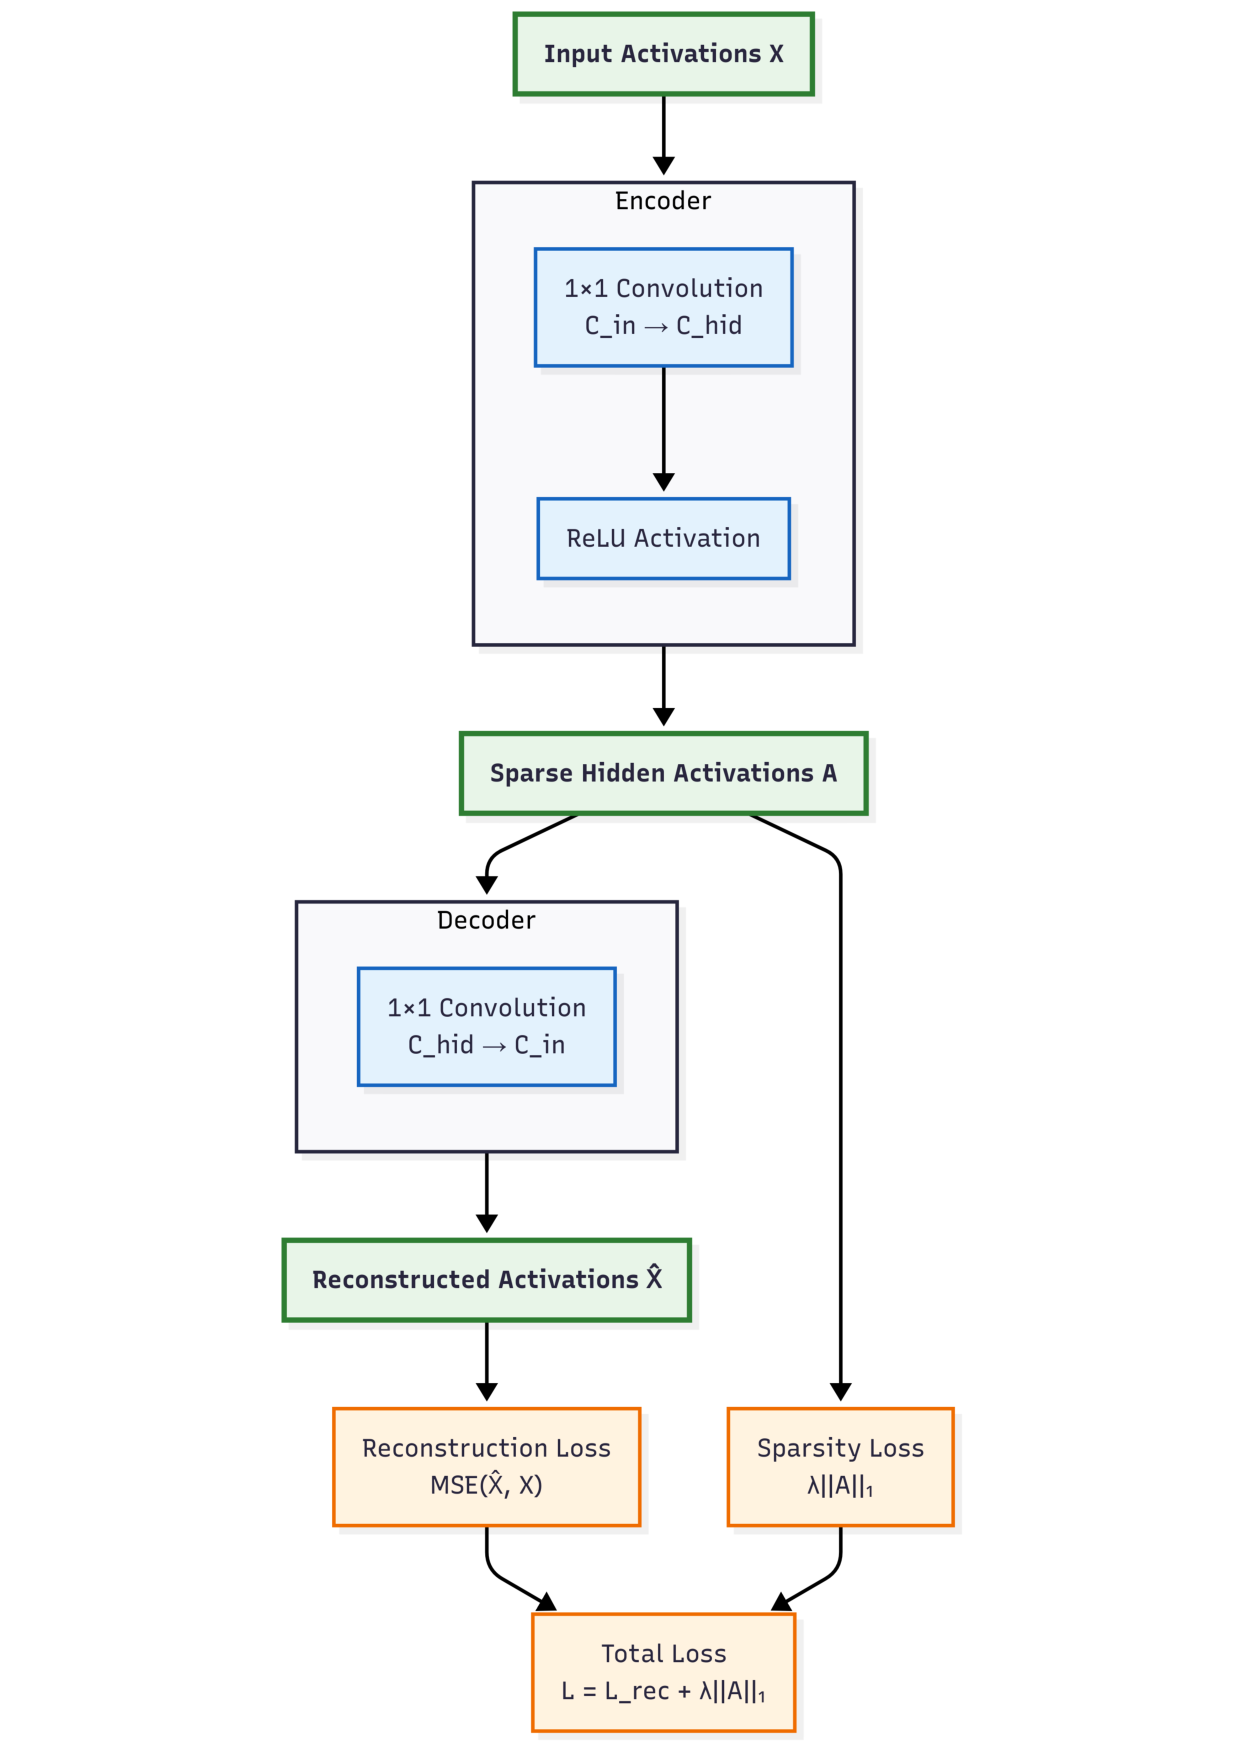
\includegraphics[width=0.8\textwidth]{figures/sae_mermaid.pdf}
    \caption{Sparse auto-encoder (SAE) architecture. An encoder applies a $1\times 1$ convolution and ReLU to map input activations $X$ to sparse hidden activations $A$; a second $1\times 1$ convolution reconstructs $\hat{X}$. Training minimises the reconstruction loss $\text{MSE}(X,\hat{X})$ plus an $\ell_{1}$ sparsity penalty $\lambda\lVert A\rVert_{1}$. \textit{Shapes:} $X\in\mathbb{R}^{B\times C_{\text{in}}\times H\times W}$, $A\in\mathbb{R}^{B\times C_{\text{hid}}\times H\times W}$, $\hat{X}\in\mathbb{R}^{B\times C_{\text{in}}\times H\times W}$.}
    \label{fig:sae_architecture}
\end{figure}

Recent approaches such as SAEs~\citep{bricken2023monosemanticity, gorton_2024_missing}, sparse probing~\citep{durrani2021transformer}, and neuron-level interventions~\citep{meng_2023_locatinga}, combat superposition by learning over-complete sparse dictionaries or low-dimensional subspaces that disentangle features and are discussed further in Section~\ref{subsec:post_hoc}. In particular, SAEs compress activations into sparse, over-complete features that split polysemantic neurons into monosemantic latents and have revealed interpretable features in both CNNs and transformers~\citep{conerly_update_2024}.


\subsection{Feature Visualization Techniques}\label{subsec:visualising_neural_networks}

Techniques such as those developed by~\citet{zeiler_2013_visualizing} represented the first work on interpreting the operations of deep neural networks. They employ a deconv-net, a model that maps feature activations from a deep layer back to the input pixel space by approximately reversing the network's pooling and convolutional operations. By reconstructing the maximally activating zones in pooling layers and being chained through subsequent CNN layers the reconstruction of complex visual representations of deep layers within the network can be achieved. This is normally very challenging due to the significant compression that is performed on the deep layers in the CNN. By applying this deconvolution the features appearing deeper in the network can be expanded back up to human interpretable scales.

Early work in understanding the functioning of neural networks focused on techniques that could visually represent the features that were encoded in the weights of the neural network. In particular, \citet{olah_feature_2017} developed techniques to generate maximally activating synthetic inputs that functioned as startlingly clear representations of channels and layers within the network. These visualisations revealed a clear hierarchy of abstraction, demonstrating how simple features from one layer (`curve-circuits') compose into more complex, semantically coherent representations (e.g., object parts) in the next. This work also demonstrated the use of gathering maximum activating samples from the training data and pairing it with particular channels and showing the similarity between these and the synthetically generated examples as a means of confirming the veracity of the visualisations.



While synthetic visualizations can be noisy, maximally activating patches, especially from within the environment, can yield interpretable results, confirming findings in~\citep{hilton_2020_understanding}. Work done on exploring SAEs trained on CNNS such as~\citep{gorton_2024_missing} makes effective use of visualisation to illustrate the improvement in interpretability of the SAE latents.


\subsection{Post-hoc Explanations}\label{subsec:post_hoc}
% Methods that explain already trained models
% Feature attribution, saliency maps, etc.

\subsubsection{Attribution and saliency methods} Post-hoc explanation methods aim to provide insights into already trained models without altering their architecture or training process. Examples include probing, SAEs, feature attribution methods (like LIME~\citep{ribeiro_2016_why}, SHAP~\citep{lundberg_2017_unified}), saliency maps~\citep{Simonyan14a,selvaraju_2017_gradcam}, and activation steering~\citep{turner_2024_steering,zou_2025_representation}.

LIME focuses on creating explainable functions by approximating a model's local behaviour around a specific input, and observing which changes create the greatest difference in the final outputs, weighting inputs by their proximity to the original input (with closer inputs being weighted more heavily). They then create a modified linear approximation that is explainable and train it on this weighted dataset which can then be more easily interpreted~\citep{ribeiro_2016_why}.

SHAP provides consistent estimations of feature importance based on Shapley values from cooperative game theory. It assigns each feature an importance value by calculating its average marginal contribution across all possible feature combinations, ensuring properties like local accuracy and consistency that other methods lack~\citep{lundberg_2017_unified}. It is quite costly to calculate however, as it requires calculating contributions over all possible feature subsets.

Saliency-based feature-attribution techniques, while originally developed for image classification, have been shown to yield insights into RL policies. These methods typically operate by computing the gradient of a relevant policy output (such as the value of a state or the probability of a specific action, $f(s)$) with respect to the input observation, $s$. The resulting saliency map is then defined as the magnitude of this gradient:
\[
    M(s) = |\nabla_s f(s)|,
\]
which highlights pixels that most strongly influence the agent's decision. Using this approach, \citet{greydanus_2018_visualizing} applied gradient saliency maps to Atari DQN agents, showing that agents frequently track critical entities like the ball in Breakout or enemy ships in Space Invaders (Figure~\ref{fig:breakout_saliency}).

\begin{figure}[htbp]
    \centering
    \includegraphics[width=0.9\textwidth]{figures/breakout_saliency.png}
    \caption{Saliency maps for a DQN agent learning to play Breakout, showing the evolution of attention patterns during training. Blue regions indicate areas most salient to the actor (policy), while red indicates areas salient to the critic (value function). Early in training, attention is diffuse; as learning progresses, the agent focuses on strategically relevant features such as the ball and the tunnel through the brick wall. Note that this figure illustrates saliency maps generally; the effect of longer rollouts on visualisation crispness discussed above is not shown here. Figure reproduced from~\citet{greydanus_2018_visualizing}.}
    \label{fig:breakout_saliency}
\end{figure}

To address the shortcomings of simple gradients, Sundararajan's integrated-gradients method\,\citep{sundararajan_2017_axiomatic}, which accumulates gradients along a path from a baseline input, was later extended to policy networks by~\citep{atrey_2020_exploratory}, who introduced `policy saliency' maps that operate over distributions of outputs from policy models. These approaches provide an easily computable and highly informative result without requiring additional training. However, unlike SAEs or steering vectors, these methods do not provide a mechanism for manipulating behaviour.

\subsubsection{Probing}\label{subsubsec:probing}
Perhaps the most famous and enduring of post-hoc techniques is probing, particularly the linear probe~\citep{alain_2018_understanding}. This is simply a linear classifier trained on activation data from a given layer on target labels that are provided based on a pre-registered target of interest. The degree of accuracy that the probe can achieve represents the degree to which a given layer can be said to contain a representation of the given target feature within the layer~\citep{alain_2018_understanding}. Deeper probes consisting of multiple layers are also a useful tool, but these can obfuscate the degree to which the target feature is actually present due to the additional computation being performed.

Probing is a core tool in mechanistic interpretability due to the wide array of situations where it can be applied and the low cost of implementation. It also reveals a great deal of information about where in the network a certain operation is being performed such as object detection, spatial reasoning, or feature composition. 

Probes have been able to provide powerful insight when applied creatively to neural networks. An excellent example of the explanatory power of probes can be found in~\citet{li_2024_emergent} which demonstrated that a model trained to produce legal moves in the game of Othello after being provided a preceding sequence of moves had a rich encoding of the board state embedded within the weights, as opposed to having learned complex heuristics to predict likely next moves. They demonstrated using non-linear probes (2 layer MLPs), that they could extract the state of the board by which types of piece occupied each square on the grid. They did this by training 64 probes in parallel, each probe being trained exclusively on the underlying ground truth data for a specific grid position across the training datasets. The ground truth data consisted of `black', `white', or `neutral' states for each position. They tried linear probes and the 2 layer probes, and found that the linear probes were able to achieve only around 20\% performance while the 2 layer probes achieved up to 98.7\% accuracy.~\citet{nanda_2023_emergent} expanded on this work by showing that in fact it was possible to achieve extremely high accuracy with linear probes, but that the ground truth data needed to be altered to represent `yours', `mine', or `neutral', and that it would swap depending on whose turn in the game it was. This demonstrated that the additional computation performed by the 2 layer probes was obfuscating the underlying representation that the model had learned.

However, probes do have significant limitations as well. They provide only correlational evidence of the purpose of what the network is doing. They may show that some activation contains the relevant information but not what it is doing with it or whether it is acting upon it. There is also a risk that probes are in fact doing computational work to construct features rather than simply revealing them, if the probes have multiple layers and many neurons. For example, an MLP probe trained to detect the presence of a cat in activation space could infer the cat from isolated features in the network that would normally only be combined later in the network. The Othello GPT example illustrates how the MLP probes were performing additional computation to adjust to the non-native representation of the board state within the activations.


\subsubsection{Sparse Probing}

Sparse probing is an approach that aims to address polysemanticity (Section~\ref{subsec:superposition}) by selecting a portion of a network, such as a channel, a layer, or multiple channels, and then training a linear classifier that uses only a subset of size $k$ neurons from that section to predict a target feature~\citep{gurnee_2023_finding}. The classifier makes predictions about the target class using only these $k$ neurons, and researchers can then observe which neurons have the highest predictive power by comparing classification accuracy. By iteratively selecting different values of $k$ and retraining, this method surfaces which neurons are most important for feature detection, and allows researchers to determine how much of the network is required for the given operation based on the accuracy scores for different sizes of $k$.

When $k=1$, this method isolates individual neurons that serve as feature detectors. Experiments across diverse architectures and tasks revealed that certain high-level semantic features achieve classification accuracies exceeding 75\% using single neurons. 
The existence of neurons with near-monosemantic responses indicates that neural networks can develop localized representations despite their distributed architecture. This localization appears most pronounced in middle layers, where abstract representations have formed but have not yet been transformed into task-specific outputs. Such neurons enable targeted interventions and provide empirical evidence that understanding can be done through analysis of individual components rather than requiring more complex distributed interventions.

Feature detection accuracy exhibits a characteristic non-monotonic pattern when varying the sparsity parameter $k$: rapid improvement for small $k$ followed by plateau or decline~\citep{gurnee_2023_finding}. This pattern indicates encoding through a small core set of highly informative units, with additional units contributing marginally or detrimentally to classification. Optimal sparsity varies systematically with feature complexity and network depth. Early layers involved with integrating low level features typically require $k\in[10,50]$ before yielding high accuracy, while later layers can peak with $k\in[1,10]$.

Sparse probing has significant limitations in that it requires significant human effort to determine the nature of the features detected with the sparse probing, and thus the field has not moved much in this direction, with unsupervised dictionary learning approaches such as SAEs becoming the preferred approach for isolating features in the network. However, sparse probing still provides significant utility in understanding smaller networks where the number of features is much fewer and target concepts can be concretely specified for probe training and especially allows for concrete understanding of the precise operations of the actual network that may be obfuscated in an SAE.

\subsubsection{Dictionary learning}\label{subsubsec:dictionary_learning}

Dictionary learning~\citep{olshausen_1996_emergence} provides a principled approach to resolving superposition (Section~\ref{sec:interpretability}). The goal is to discover an overcomplete dictionary $D \in \mathbb{R}^{d \times k}$ (where $k > d$) whose columns serve as basis vectors that can represent input data $x \in \mathbb{R}^d$ through sparse linear combinations:
\[ x \approx D \cdot \alpha, \]
where $\alpha \in \mathbb{R}^k$ is a sparse coefficient vector. Unlike standard bases that require exactly $d$ linearly independent vectors, dictionary learning trades redundancy (overcomplete basis) for sparsity (each data point activates only a few basis vectors). This sparse, distributed representation disentangles features that would otherwise be superposed in the original $d$-dimensional space, as described by Equation~\ref{eq:superposition}.

Classical algorithms such as K-SVD~\citep{aharon_2006_ksvd} and FISTA~\citep{doi:10.1137/080716542} solve this optimisation problem through iterative sparse coding and dictionary updates. SAEs provide a neural network approach to this same objective.

\subsubsection{Sparse AutoEncoders}\label{subsubsec:SAEs}

SAEs utilise neural networks to perform unsupervised discovery of the dictionary. This provides a sparse encoding of the original features of the model (which we refer to as latents in the SAE), which arise due to the enforcement of a sparsity penalty applied during the training of the SAE. SAEs aim to faithfully reconstruct the activations of a given layer in a network while keeping their own internal activations sparse. The training objective is therefore to find encoder and decoder weights that minimise a loss function combining a reconstruction term and a sparsity term, which typically takes the form:
\[L(x) = \|x - \text{Dec}(\text{Enc}(x))\|_2^2 + \lambda \|\text{Enc}(x)\|_1\]
Here, \(x\) represents the original activation from the base model, the L2 norm penalizes poor reconstruction, and sparsity is enforced by minimising the product of the L1 norm of the SAE's internal activations, and a coefficient \(\lambda\)\citep{bricken2023monosemanticity}.  

SAEs typically learn an overcomplete basis, where the hidden layer of the SAE is much larger than the original layer it is reproducing, typically chosen by multiplying the original hidden dimension size by some expansion factor. This high dimensionality allows the SAE to represent the input activations using a small number of highly specific, disentangled features. This addresses the problem of polysemantic `units' in a model, which can make the task of accurate interpretability much more challenging~\citep{elhage2022superposition}.

The direct methodological precedent for applying SAEs to convolutional networks comes from recent work by \citet{gorton_2024_missing}, who successfully trained SAEs on the InceptionV1 image classifier. Their approach uses a `1x1-conv SAE' architecture, as illustrated in Fig~\ref{fig:sae_architecture}. An encoder with a learnable $1\times1$ kernel maps the input activation tensor $X$ to a sparse, high-dimensional hidden activation tensor $A$, which a symmetric $1\times1$ decoder then uses to reconstruct $\hat{X}$. To train this effectively on CNNs, they introduced several key innovations. First, to manage computational cost, they used \emph{activation oversampling}, preferentially sampling training data from spatial locations with high activation magnitudes to focus on learning meaningful features rather than background noise. Second, they used highly over-complete dictionaries, with expansion factors up to 8, to provide the capacity needed to disentangle features. The results were compelling: their SAEs successfully split known polysemantic `double-curve' units in InceptionV1 into distinct monosemantic features and recovered a suite of previously `missing' curve detectors. These findings provide concrete evidence that dictionary-learning SAEs can resolve superposition in CNNs and motivate their application to RL agents with convolutional backbones.

To formalise the above concept, let $a^{l}(x)\in\mathbb{R}^{d}$ be the activations of layer $l$ for input $x$, and let $w\in\mathbb{R}^{d}$ be the extracted weight vector of the linear classifier trained to distinguish positive concept examples from counter-examples.  We take the concept activation vector as
\[
    v^{l}_{C}= \frac{w}{\lVert w \rVert_{2}}.
\]
Following~\citet{gorton_2024_missing}, the extent to which concept $C$ influences the logit $f_{k}(x)$ for class $k$ is measured by the directional derivative
\[
    S_{C,k,l}(x)= \nabla_{a^{l}(x)} f_{k}(x) \cdot v^{l}_{C},
\]
whose sign indicates whether amplifying the concept increases ($S_{C,k,l}>0$) or decreases ($S_{C,k,l}<0$) the likelihood of a particular prediction.

Because these can be learned with a lightweight linear probe and then used to potentially intervene on neural network activations as illustrated in work such as Othello GPT~\citep{nanda_2023_emergent}, this technique has become fundamental as a tool in alignment~\citep{meng_2023_locatinga}, and lays a conceptual foundation for things like steering vectors, which are produced in a different way but share many properties~\citep{turner_2024_steering}.


The feature visualization methodologies discussed, such as synthetic visualization (optimizing an input image for maximal channel activation) and finding maximally activating dataset samples~\citep{olah_feature_2017,hilton_2020_understanding}, are also forms of post-hoc analysis.


\subsubsection{Concept Activation Vectors} 
Concept Activation Vectors (CAV) provide a way to bridge the gap between the high dimensional vector space of neural network activations and human-understandable concepts. To construct a CAV for a concept (`striped'), one collects a small set of images that exhibit the concept and a set of random counter-examples, records the activations from a chosen layer, and trains a linear classifier to separate the two groups. The normal vector to the resulting decision boundary is the CAV. This can then be manipulated in one direction or the other to produce more or less of the effect you desire~\citep{kim_2018_interpretability}. This can be used to test how much a particular concept is relied upon when the network is making a prediction. Recent applications of CAVs have shown promising results in debugging vision models and identifying spurious correlations in training data.

\subsubsection{Activation Steering}\label{subsubsec:activation_steering}
Activation steering, as demonstrated in~\citet{mini_2023_understanding,turner_2024_activation} discussed further in Section~\ref{sec:Understanding}, is another post-hoc technique. Steering typically makes use of CAVs, captured by using the difference in activations between states with and without a particular characteristic, can be used to influence a policy model's behaviour by acting as a superstimulus for particular environmental aspects. This is achieved through the transformation $h^{l'} = h^l + \alpha \cdot v^l$, where the steering vector $v^l$ is added to the original activations $h^l$, with $\alpha$ modulating the intervention strength. The steering vector itself is computed as $v^l = \mathbb{E}[h^l|\text{with target}] - \mathbb{E}[h^l|\text{without target}]$, capturing the difference in activations when the target is present versus absent.

In language models (LMs) a typical approach used to do activation steering is to use contrastive pairs~\citep{turner_2024_activation}. In this approach one presents two different segments of text that are identical in every way except one, for example one may pass the following two inputs through an LM and then calculate the mean across the activations of the tokens and then calculate the difference in the two mean values to capture the `speak in French' concept vector, which can then be used to steer the model to speak in French or English by modifying $\alpha$ to be positive or negative and adjusting its magnitude. This is normally done across many samples, with the mean of those pairs being used for steering. 
\begin{itemize}
    \item \textbf{English:} ``The teacher explained the complex problem using simple examples.''
    
    \item \textbf{French:} ``L'enseignante a expliqué le problème complexe en utilisant des exemples simples.''
\end{itemize}

Activation steering is an excellent tool for interpretability due to the ease and speed with which it can be used, and because it allows researchers to immediately observe how a network responds to a specific concept being made more or less prominent in the forward pass of the network. They also allow researchers to determine whether a concept exists and is easily representable in given layer of a network. Given that you can extract concept from single layers, or multiple layers simultaneously, one can test whether the concept is meaningful within a certain part of a network by the degree of change in output observed by its application there.

\subsection{Intrinsically Interpretable Models}\label{subsec:intrinsic}
Intrinsically interpretable models are designed from the outset to be understandable, often by constraining their complexity (e.g., linear models, decision trees) or by building in mechanisms that are inherently transparent. Training SAEs can be seen as an effort to transform parts of a complex model into a more intrinsically interpretable representation by disentangling features.

Many existing interpretability techniques were developed for supervised settings with i.i.d.~data. Reinforcement learning violates many of these assumptions. For example, observations are generated by an agent acting in, and affecting, a dynamic environment, and credit must be assigned across time. As a result, many tools require adaptation to work within this paradigm. The next section explores some techniques that have been developed explicitly to overcome this gap.

\subsection{Causal Methods in Interpretability}\label{subsec:causal}

Many of the techniques discussed in the methodology, such as activation steering (Section~\ref{subsubsec:activation_steering}), can serve dual roles as both post-hoc explanation tools and causal testing methods when applied systematically. This section focuses on additional causal techniques and frameworks for rigorous causal claims in interpretability research. These techniques actively modify the operations of the network, testing whether specific components are genuinely responsible for behaviours of interest~\citep{10.5555/1642718}.

Modern systematic ablation has evolved through several generations. Zero ablation, the simplest approach, sets components to zero but can lead to out-of-distribution behaviours since networks rarely encounter zero values during training. Mean ablation, which replaces components with their average values across a sample dataset, better preserves activation statistics but may incompletely remove information if the mean itself carries useful information. Recent work~\citep{li_2024_optimal} introduces optimal ablation constants that are computationally determined to minimise the expected loss on the task, reducing the amount of distributional shift in the final outcome.

Work on finding induction heads in neural networks~\citep{olsson_2022_incontext} is a prime example of rigorous systematic ablation. In this work they thoroughly demonstrated causality via targeted removal. Their task setup involved identifying how LMs were able to successfully complete simple A-B pattern matching, meaning that when a pattern of B following from A was observed the model should repeat this pattern when a later example of A was shown. When induction heads were ablated in small models, in-context learning collapsed from near-perfect to near-random on the task of A-B pattern matching. This showed that induction heads were essential for this task.

For agents with spatial convolutional representations, targeted synthetic interventions can directly test the functions of parts of the network by intervening on their values directly.~\citet{mini_2023_understanding} demonstrated that clamping a single activation in a channel that typically identified the location of the cheese (channel 55) to a large positive value at a specific location in the maze could steer the agent to that location, as if that was the final goal of the maze. This provided direct causal evidence that this channel had an unusual ability to steer the direction of the agent.

These causal techniques provide the foundation for the experimental methodology employed in this thesis. Systematic ablation is used to test the necessity of individual SAE channels for navigation (Section~\ref{sec:expanded_ablation_methodology}), while activation interventions combined with behavioural testing establish sufficiency of specific channels for steering agent behaviour (Section~\ref{subsubsec:steering_interventions}). Together, these approaches move beyond observation to establish genuine causal mechanisms underlying goal representation in RL agents.


\section{Interpretability in Reinforcement Learning}\label{sec:rl_interpretability}

Interpretability in RL presents unique challenges due to the agent's interaction with an environment, the fact that specific outputs of the model might be extremely semantically distant from the contents of a given activation, and because we can only infer the meaning of a given observation of an activation within the model, we can't directly glean it as we could a word extracted from the embedding space of a language model.

Recent research shows that such models naturally learn geographic mappings of the world related to locations that can be retrieved directly from the activations of the network, effectively building simplified world models~\citep{gurnee2023language}. Similarly, analyses of agents trained on complex games like chess demonstrate that these systems acquire human-understandable strategic concepts, such as piece values or tactical motifs, purely from self-play~\citep{mcgrath_2022_acquisition}. These findings suggest that the internal workings of these models are richer than previously thought and lend support to the idea that they plausibly learn to represent goals that can be directly extracted from the model and understood. As illustrated in Figure~\ref{fig:environment-overview}, even a seemingly simple maze can embed multiple, dynamically changing goals whose representations the agent must learn to use effectively.

Work by~\citet{betley_2023_localizing} found a specific circuit in the convolutional layers of the Impala model that activated strongly when the direction to go was `up' and didn't activate when the goal was in a similar position but the agent would need to go in a different direction. This indicates that much of the `planning' was already performed in the CNN layers, suggesting it should be possible to train probes that can detect the exact direction the agent needs to move towards.

Work exploring the Procgen Coinrun environment builds on saliency based methods (Section~\ref{subsec:post_hoc}) to calculate an attribution within the model weights themselves. By measuring the contribution of a given convolutional feature map to the value function, it becomes possible to determine if a particular feature that the model is observing is likely to have a positive or negative effect on the success of the model, based on whether the collected gradient multiplied by the activation score is positive or negative. This advances previous saliency mapping methods by linking the gradients to specific features within the model, rather than pixels in the input~\citep{hilton_2020_understanding}.

This is achieved by applying non-negative matrix factorisation (NMF) of the attribution tensor to cluster correlated locations across channels into object-level `features' such as coins, enemies, obstacles etc. By using this dimensionality reduction they are able to produce clear, interpretable object detectors. 



% To provide a precise explanation of this process, let $X^{(n)}\in\mathbb{R}^{C\times H\times W}$ be the activation tensor of a convolutional layer for input $n$ and let $V^{(n)}$ be the value head.  Element-wise product of activation and gradient attribution is
% \[
% A^{(n)}_{c,h,w}=X^{(n)}_{c,h,w}\;\frac{\partial V^{(n)}}{\partial X^{(n)}_{c,h,w}}.
% \]
% Flatten $A^{(n)}$ to a vector $a^{(n)}\in\mathbb{R}^{D}$ with $D=CHW$ and stack $N$ such vectors into a matrix $R\in\mathbb{R}^{N\times D}$. This results in an $N \times D$ matrix where each row is a single observation, and each column is a `feature location'. We then apply NMF to this matrix, keeping $A^{(n)+}_{c,h,w}=\max\bigl(0, A^{(n)}_{c,h,w}\bigr)$ to satisfy the non-negativity constraint. Non-negative matrix factorisation seeks
% \[
%     R\;\approx\;W H,\quad W\in\mathbb{R}_{\ge0}^{N\times r},\;H\in\mathbb{R}_{\ge0}^{r\times D},
% \]
% with a small rank $r$. Each row of $H$, reshaped back to $(C,H,W)$, yields a sparse mask that acts as a detector for in-game entities (coin, enemy, hazard). 



\section{Understanding and Controlling a Maze Solving Policy Network}\label{sec:Understanding}
Previous work by~\citep{mini_2023_understanding} demonstrated the ability to manipulate an agent's navigation in a simple maze environment with an intervention to a single channel in the network, providing the primary motivation for this work with the intent of extending these techniques to more complex multi-objective settings. The work specifically used an agent which had been trained in a modified version of the environment where the cheese was only ever added to the top right of the environment, and then deployed the agent into settings where the cheese could spawn at any location in the maze. This meant that there was a tension between the agent's natural tendency to want to go to the top right of the environment and to go the cheese location.

They go on to show that the agent's decision making about whether it travelled to the top right or towards the cheese alone was determined by both the Euclidean distance between the agent and the cheese and the path distance between the agent and the cheese. This means that the agent had multiple separate mechanisms driving its decisions rather than being a single unified policy. They did this by showing through regression analysis that if the agent was an equal path distance from two instances of cheese, it would tend to approach the cheese that was also closer in Euclidean distance. 

This shows a surprising contradiction in the agent because Euclidean distance should not meaningfully affect a maze-solving policy (the agent cannot walk through walls), suggesting the agent is not relying on a single reward-maximising policy but is instead operating under multiple competing goals.

They further demonstrate that neural networks can develop interpretable mechanisms to track goals. The authors identified specific channels that tracked the location of objectives in a maze environment and showed that these could be manipulated to control the agent's behaviour. They found that steering vectors, the difference in activations between otherwise identical states with and without an entity, could be used to influence the model's behaviour in predictable ways. This work serves as the foundation for our research, though we extend it to a multi-objective setting.

Recent concurrent work by~\citet{trim_2024_mechanistic} extends the work done by~\cite{mini_2023_understanding} to analyze goal misgeneralization. Their layer-by-layer analysis reveals a hierarchy of representations: early layers (b1.conv) detect basic features such as walls, paths, and the cheese goal; middle layers develop more abstract concepts including possible `flood fill' patterns for directional pathways; while deeper layers create highly abstracted representations where identifying the goal becomes challenging. They further confirm the positional bias seems to exist regardless of the position of the final goal within the maze, indicating a deeply learned tendency towards this direction, rather than the result of a perceptual error.

\subsection{Discovering and Controlling Goal Representations}
The authors successfully isolated the network's representation of the `cheese' goal and demonstrated causal control over the agent's behaviour. First, they defined a `cheese vector' by taking the difference in mean activations at a specific layer between trajectories where cheese was present and those where it was not:
\[
v_{\text{cheese}}^{l} = \mathbb{E}_{s \sim \text{traj}_{\text{cheese}}}[\text{act}^{l}(s)] - \mathbb{E}_{s \sim \text{traj}_{\text{no-cheese}}}[\text{act}^{l}(s)]
\]
Adding this vector back into the network's forward pass, scaled by a coefficient $\alpha$, allowed them to controllably amplify or suppress the agent's cheese-seeking behaviour.

Their most significant contribution was demonstrating this control causally through \emph{activation patching}. They intervened on the final convolutional layer of the policy network by copying the activation pattern from a small spatial region of a channel corresponding to a real cheese location and `pasting' it into the same channel at a different, empty location. By doing this they could reliably steer the agent to the empty location as if the cheese were there.

This effect was highly localized. They identified that out of 16 channels in the layer, just 11 were responsible for this behaviour. Ablating these "cheese channels" destroyed the agent's ability to find the cheese, while leaving other navigational capabilities intact. This proves that goal representations can be sufficiently modular and concentrated to allow for targeted manipulation, motivating the use of more advanced techniques like SAEs to further dissect these representations in a more complex, multi-objective setting.


\section{Gaps in the Literature}\label{sec:gaps}
Prior to the research detailed in the accompanying papers, several areas in RL interpretability remained open for exploration:

\begin{itemize}
    \item Understanding how RL agents track and switch between multiple objectives, especially when those objectives are not the immediate next target.
    \item The application and efficacy of techniques like SAEs for disentangling representations specifically within RL agent architectures, particularly CNNs.
    \item Investigating how different aspects of neural network activation encode useful information for the next layer such as how activation strength within a channel might encode information like entity identity.
    \item The role and potential utility of `dead' channels in SAEs for interpretability, which cease to activate during normal operation but might retain learned decoder weights.
    \item The generalisation of interpretability findings from simpler RL agents to more complex architectures like decision transformers or RNN-based agents, especially for tasks requiring memory.
\end{itemize}

\section{Summary}\label{sec:lit_summary}
Prior work shows huge potential in the applications of RL agents due to their ability to achieve superhuman performance generalise broadly. However, the opacity of how this is achieved represents a persistent problem. A resurgence of interest in this area due to its application in frontier AI models adds urgency to better understand these models and how they operate on a mechanistic level~\citep{mini_2023_understanding,hilton_2020_understanding}. Techniques such as activation analysis, steering vectors, and feature visualization have provided initial windows into these systems. However, challenges like polysemanticity (where neurons or channels respond to multiple unrelated concepts~\citep{olah_2020_zoom,elhage2022superposition}) and the distributed nature of representations often make it challenging to make strong conclusions about the operation of the neural network.

The application of tools like Sparse Autoencoders offers a potential solution for being able to make confident statements about whether the nature of how models truly learn to encode concepts~\citep{elhage2022superposition,bricken2023monosemanticity}, potentially making the functional roles of different network components clearer. While much of the early MI work focused on LLMs, applying and adapting these techniques to RL, with its emphasis on clear goals and environments with fewer components and potentially broadly generalisable solutions offers the ability to make unique insights that may apply to ML models more broadly.

The research presented in the accompanying papers (forming the basis of this thesis) builds directly on this existing work by:
\begin{itemize}
    \item Extending activation steering and intervention techniques to more complex, multi-objective RL environments like Procgen Heist.
    \item Applying Sparse Autoencoders to the convolutional layers of an RL agent to disentangle features and investigate the extent to which multiple entities are truly captured within a single layer of the model and through what mechanism this is done. 
    \item Systematically analyzing the role of individual channels in navigation and goal pursuit through methods like ablation studies and retargeting interventions.
    \item Exploring novel mechanisms of information encoding, such as multiplexing entity information within a single channel through varying activation strengths.
\end{itemize}
These contributions aim to deepen our understanding of how RL agents represent and pursue goals, and to refine the tools available for mechanistic interpretability for use in this domain.